\chapter{Concluzii}

% ============================================================================================================
\section{Performanță}
% ============================================================================================================
\begin{figure}[ht]
    \centering
    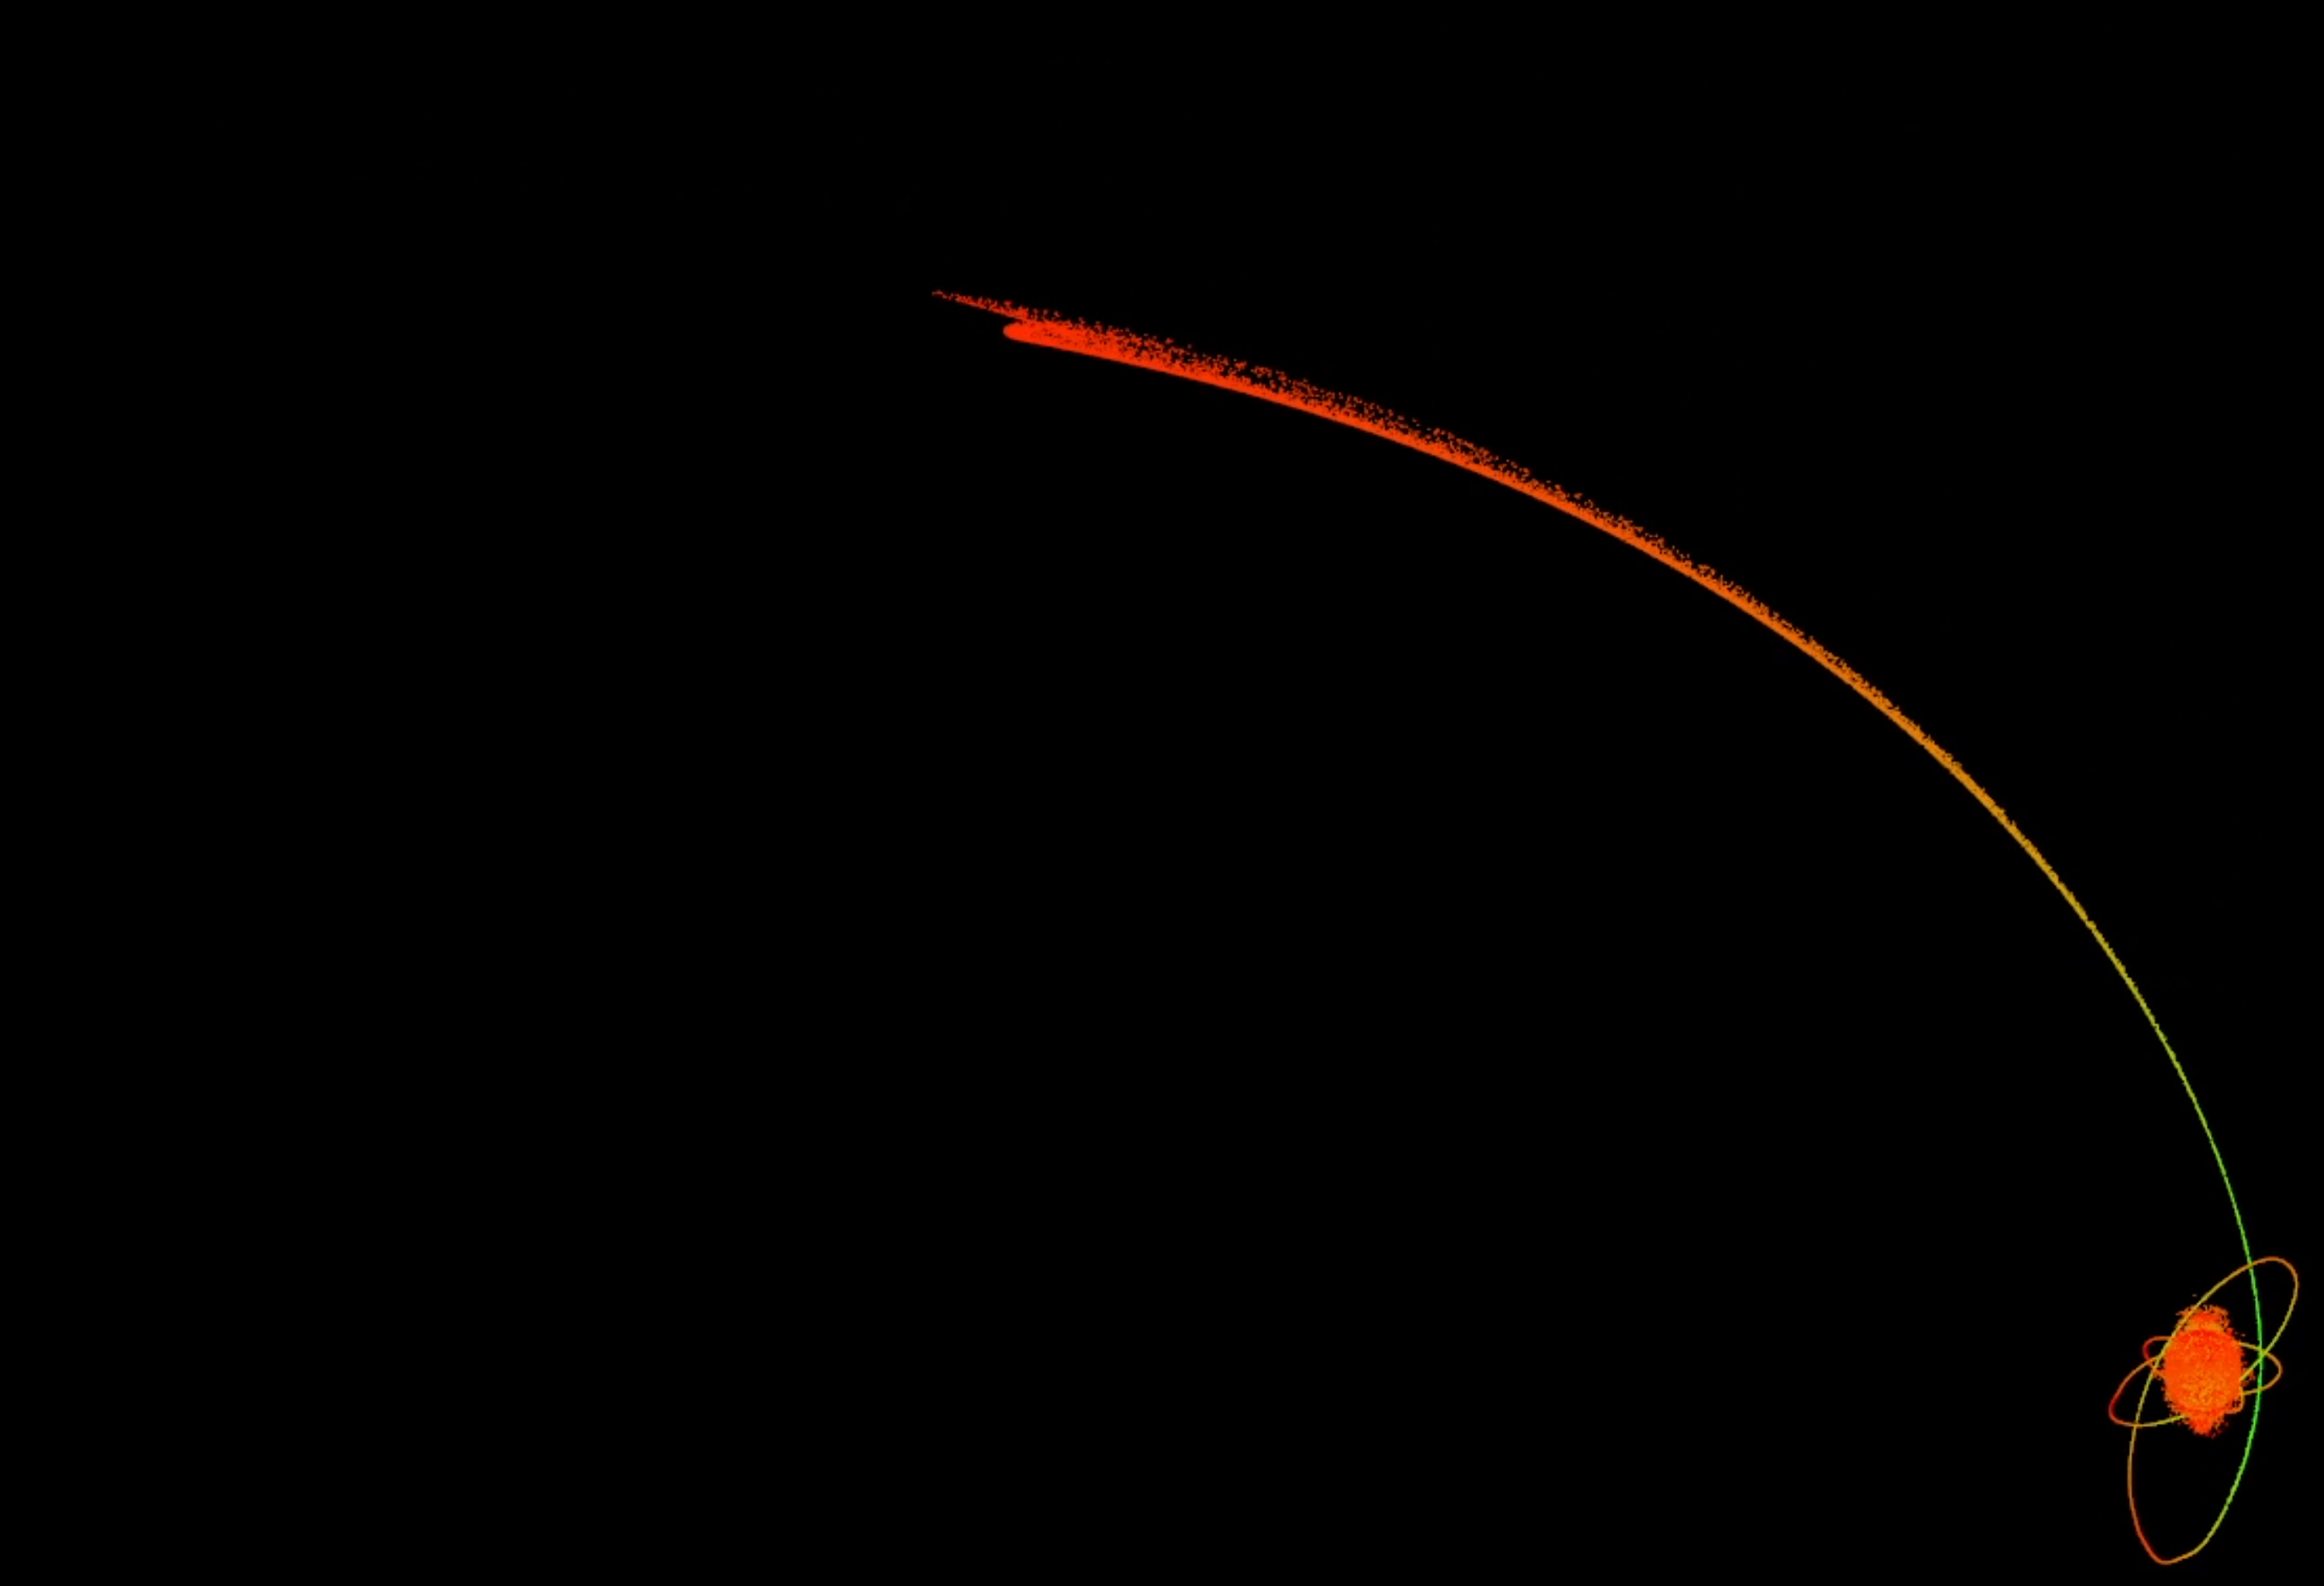
\includegraphics[width=0.8\textwidth]{images/benchmark-1.png}
    \caption{Vizualizare Benchmark 1 - 8.388.608 particule}
    \label{fig:benchmark-1}
\end{figure}

În acest capitol voi prezenta rezultatele obținute de sistemul de particule folosind diferite configurații hardware și sisteme de operare, Windows 10/11, respectiv Ubuntu 24.04.2. Evalurările testelor realizate pot oferi o perspectivă interesantă asupra modului în care sistemele de operare gestionează resursele și rularea aceleiași aplicații. Pe lângă analiza directă dintre cele două sisteme de operare, voi introduce și comparații între diferite tipuri de configurații hardware pentru a putea înțelege scalabilitatea, performanța și adaptabilitatea sistemului de particule. Pentru a putea acoperi diferite scenarii de utilizare și rendering vom folosi două benchmark-uri. Benchmark 1 (\autoref{fig:benchmark-1}) simulează 8.388.608 de particule, în care majoritatea dintre ele sunt concentrate în poziția centrului de atracție. Benchmark 2 (\autoref{fig:benchmark-2}) simulează 8.388.608 de particule, în care ele sunt cât mai răspândite, acoperind aproape întreaga suprafată de vizualizare. 

\begin{figure}[ht]
    \centering
    \includegraphics[width=0.8\textwidth]{images/benchmark-2.png}
    \caption{Vizualizare Benchmark 2 - 8.388.608 particule}
    \label{fig:benchmark-2}
\end{figure}

Prima comparație constă în prezentarea rezultatelor celor două benchmark-uri rulate pe Windows 11 (\autoref{fig:1060-windows-test-1}, \autoref{fig:1060-windows-test-2}) și Ubuntu 24.04.2 (\autoref{fig:1060-linux-test-1}, \autoref{fig:1060-linux-test-2}), ambele având aceeași configurație hardware: procesor Intel i5-8400 4.0 GHz, 16 GB RAM DDR4 2400 MHz CL15, NVIDIA GTX 1060 6 GB GDDR5 cu Boost Clock 1759 MHz. În Benchmark 1 se poate observa că aplicația pe Windows a avut o performanță per total puțin mai bună decât pe Ubuntu, FPS-ul mediu fiind mai mare pe Windows, dar experiența pe Ubuntu este mult mai stabilă, neavând la fel de multe spike-uri de performanță ca Windows. Comportamentul descris este confirmat și prin valorile minime ale FPS-urilor, diferența fiind de 8 FPS în defavoarea versiunii de Windows. De asemenea, se poate observa că în momentul în care este procesată și afișată aceeaşi imagine, versiunea de Ubuntu are cu aproape 9 FPS mai mult decât cea de Windows. În Benchmark 2 se păstrează tendințele înregistrate în Benchmark 1, cu observația că pe Windows s-a atins un număr maxim de FPS cu mult peste valoarea de pe Ubuntu. Din nou, acest efect susține afirmația că Windows este capabil de a atinge performanțe mai bune ca Ubuntu, dar nu într-un mod constant. 

\begin{figure}[ht]
    \centering
    \begin{minipage}[b]{0.48\textwidth}
        \centering
        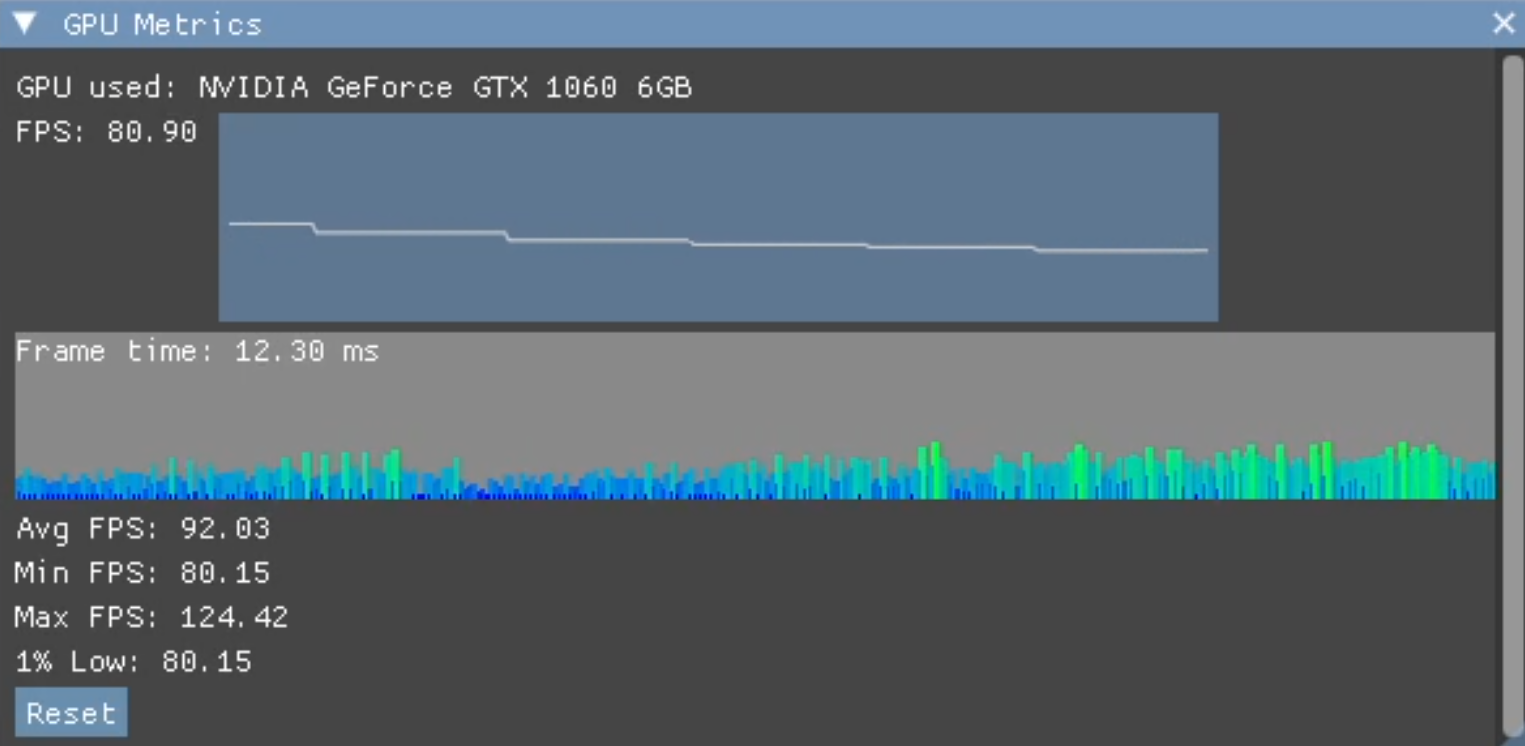
\includegraphics[width=\textwidth]{images/windows-1.png}
        \caption{Windows Benchmark 1 \\ \hspace*{6em} GTX 1060 6GB}
        \label{fig:1060-windows-test-1}
    \end{minipage}
    \hfill
    \begin{minipage}[b]{0.40\textwidth}
        \centering
        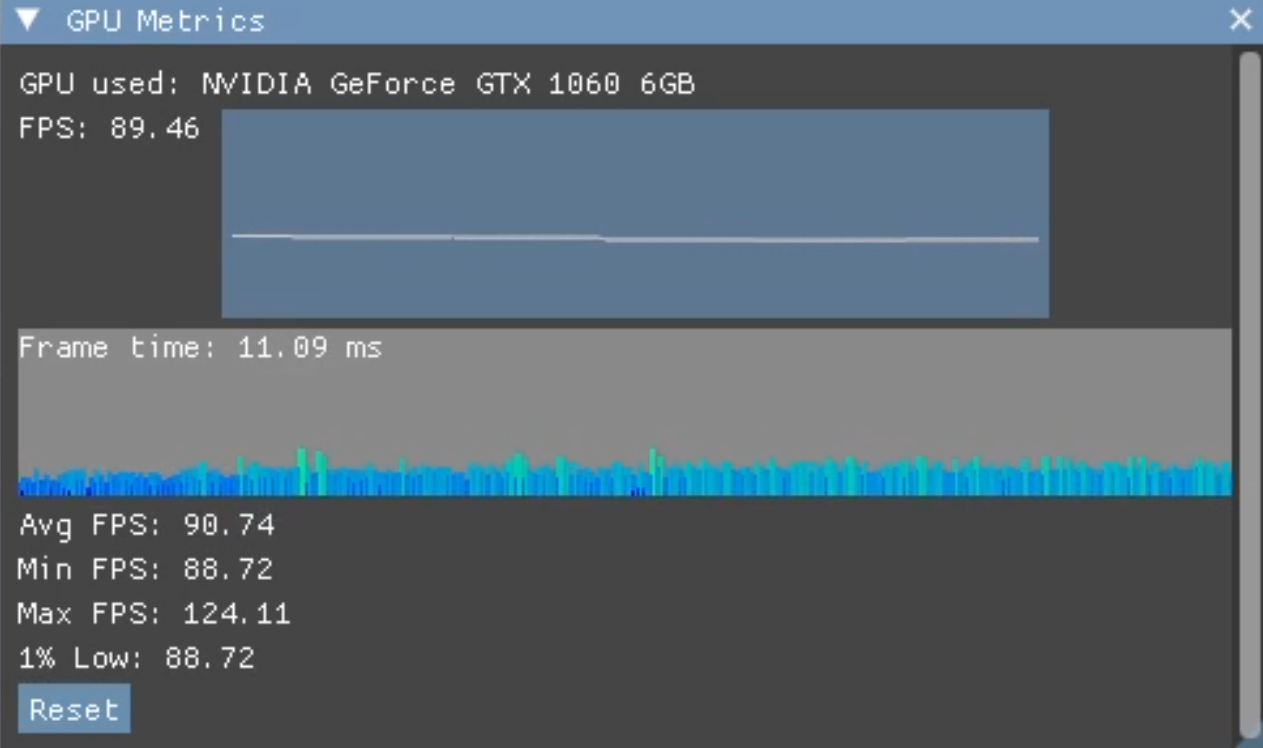
\includegraphics[width=\textwidth]{images/linux-1.png}
        \caption{Ubuntu Benchmark 1 \\ \hspace*{6em} GTX 1060 6GB}
        \label{fig:1060-linux-test-1}
    \end{minipage}
\end{figure}

\begin{figure}[ht]
    \centering
    \begin{minipage}[b]{0.48\textwidth}
        \centering
        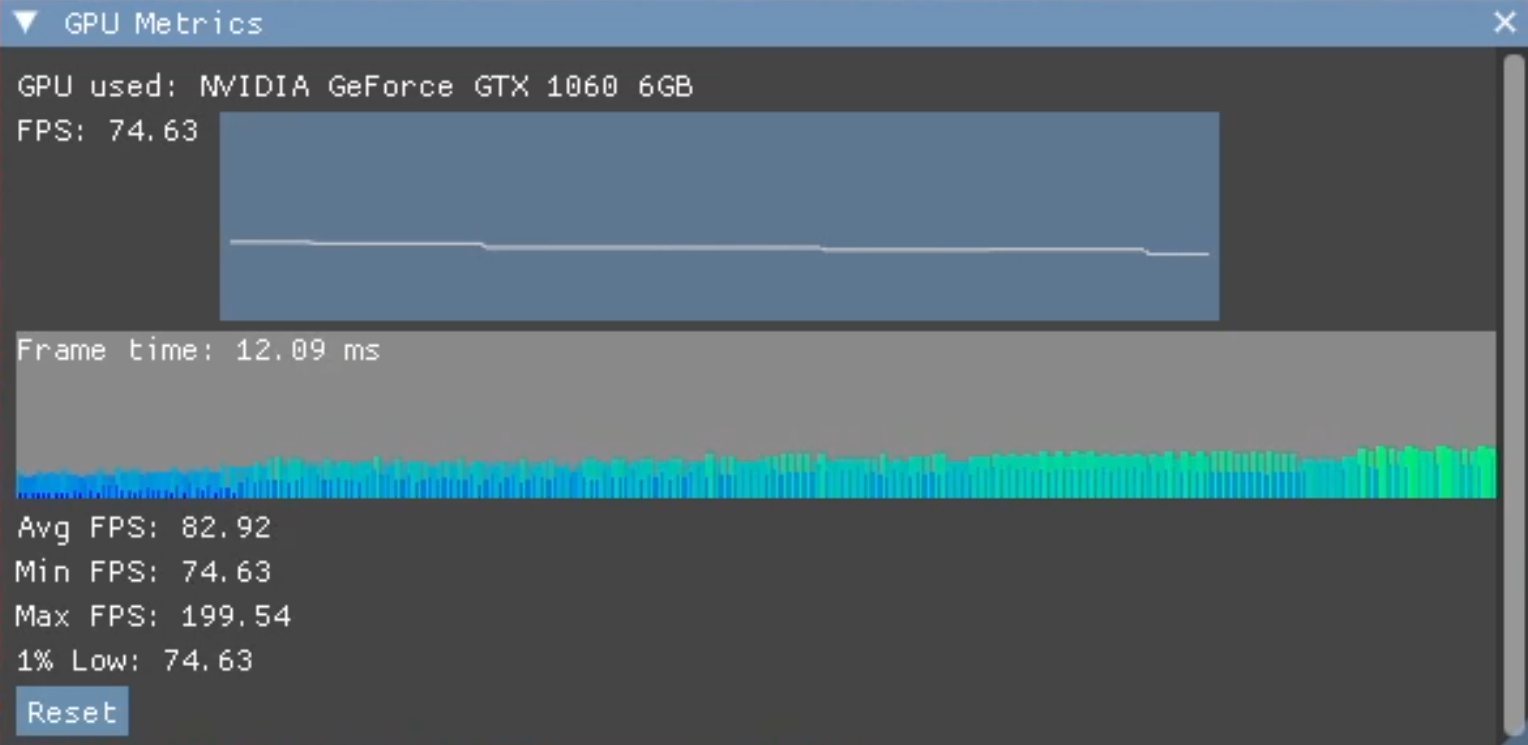
\includegraphics[width=\textwidth]{images/windows-3.png}
        \caption{Windows Benchmark 2 \\ \hspace*{6em} GTX 1060 6GB}
        \label{fig:1060-windows-test-2}
    \end{minipage}
    \hfill
    \begin{minipage}[b]{0.40\textwidth}
        \centering
        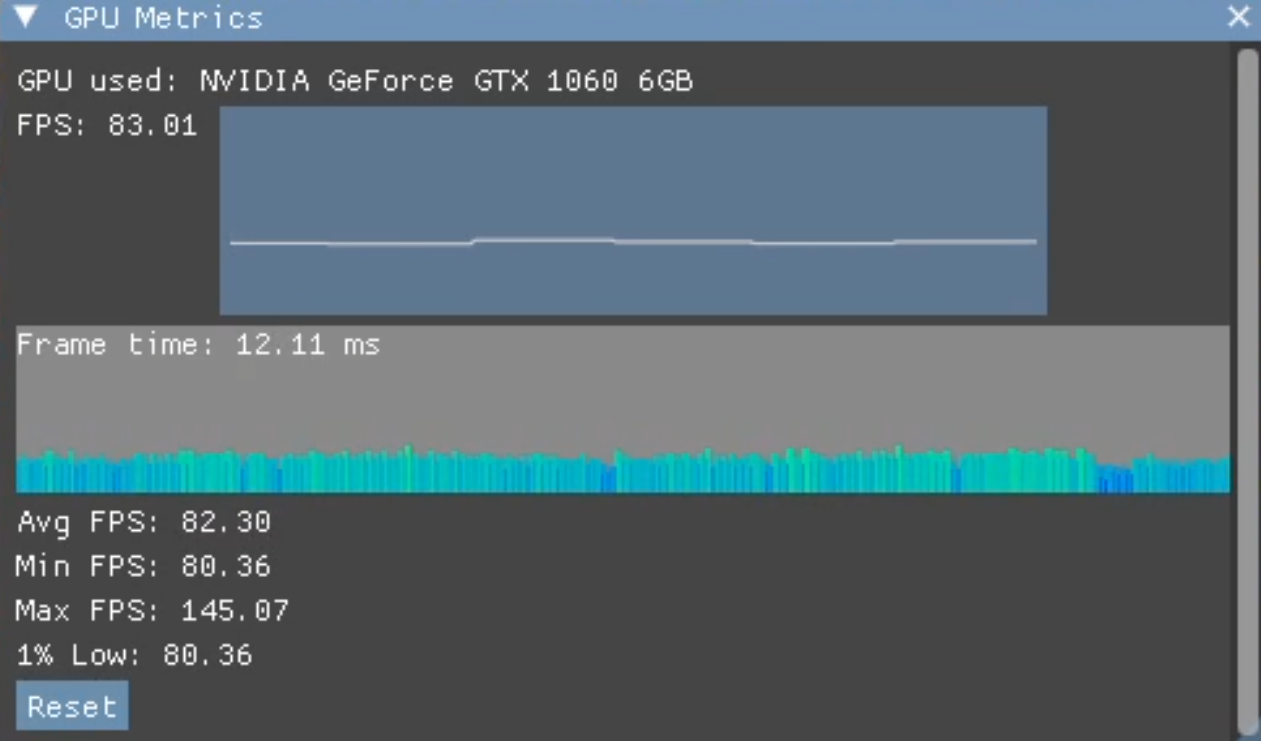
\includegraphics[width=\textwidth]{images/linux-3.png}
        \caption{Ubuntu Benchmark 2 \\ \hspace*{6em} GTX 1060 6GB}
        \label{fig:1060-linux-test-2}
    \end{minipage}
\end{figure}

A doua comparație constă tot în prezentarea rezultatelor celor două benchmark-uri rulate pe Windows 11 (\autoref{fig:5080-windows-test-1}, \autoref{fig:5080-windows-test-2}) și Ubuntu 24.04.2 (\autoref{fig:5080-linux-test-1}, \autoref{fig:5080-linux-test-2}), dar cu o configurație hardware foarte performantă: procesor AMD Ryzen 7 9800X3D 5.2 GHz, 32 GB RAM DDR5 6000 MHz CL30, NVIDIA RTX 5080 16 GB GDDR7 cu Boost Clock 2640 MHz. Se observă că tendințele din prima comparație se păstrează, versiunea de Windows oferă performanțe mai bune decât cea de Ubuntu, și sunt diminuate acele spike-uri de performnță prezente pe prima configurație hardware. Noua configurație oferă un suport mult mai stabil față de cea precedentă, fapt ce se poate datora noilor implementări atât la nivel hardware, cât și software. De asemenea, față de configurația anterioară, acest sistem oferă performanțe de până la trei ori mai mari. Este o diferență uriașă justificată în mare parte de avansul tehnologic al plăcilor video. GTX 1060 a apărut în anul 2016, iar RTX 5080 a apărut în anul 2025, o diferență de 9 ani însoțită de progres și invenții noi. Raportat la sistemul de particule dezvoltat, acest aspect nuanțează că odată cu creșterea performanței, implementarea se va folosi de toate resursele disponibile pe care le poate oferi placa video. Cu trecerea timpului, aplicația va rămâne relevantă pentru că se adaptează odată cu hardware-ul, reflectând în mod direct performanța oricărui dispozitiv. 

\begin{figure}[ht]
    \centering
    \begin{minipage}[b]{0.48\textwidth}
        \centering
        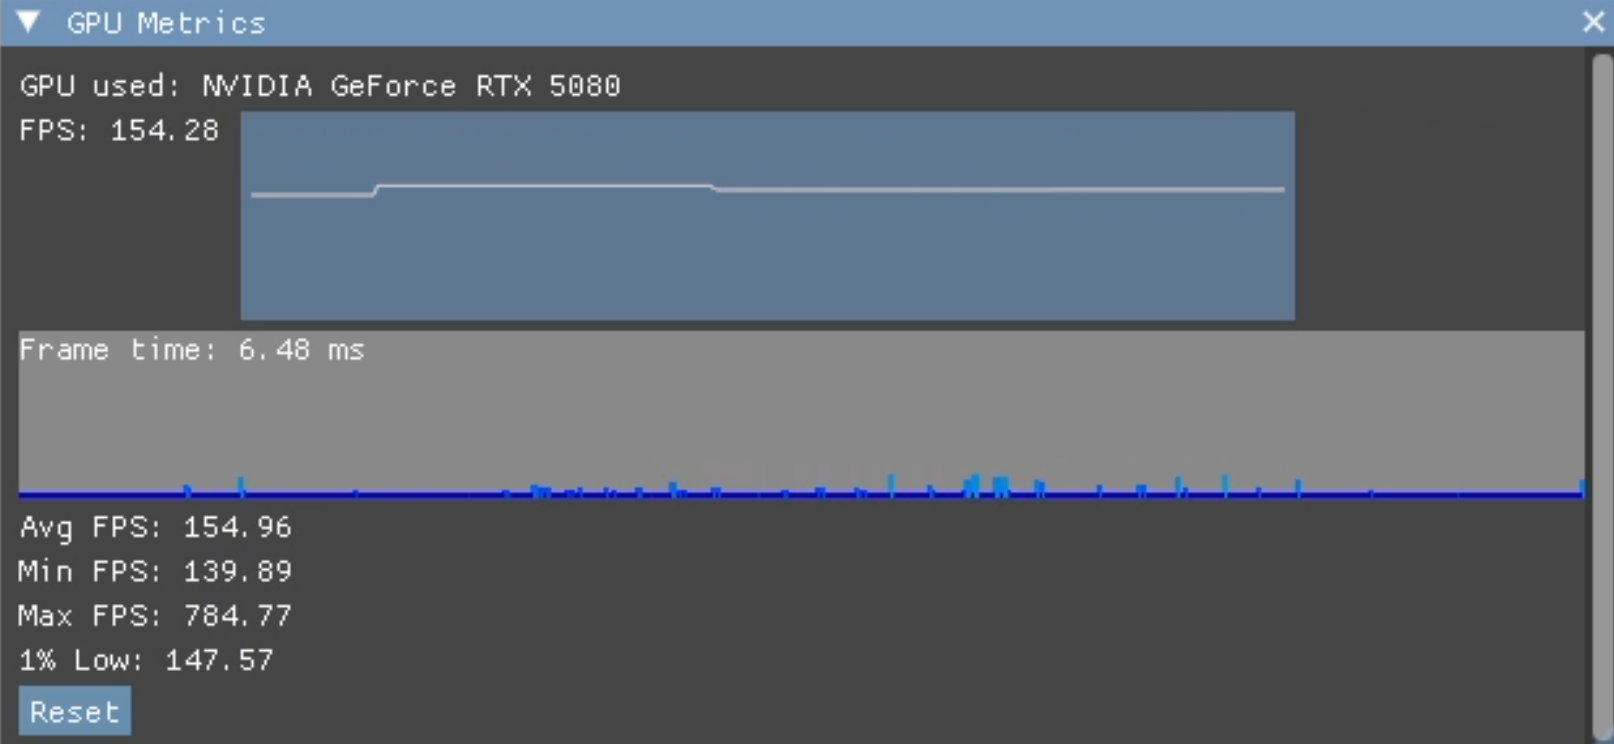
\includegraphics[width=\textwidth]{images/5080-windows-1.png}
        \caption{Windows Benchmark 1 \\ \hspace*{6em} RTX 5080 16 GB}
        \label{fig:5080-windows-test-1}
    \end{minipage}
    \hfill
    \begin{minipage}[b]{0.48\textwidth}
        \centering
        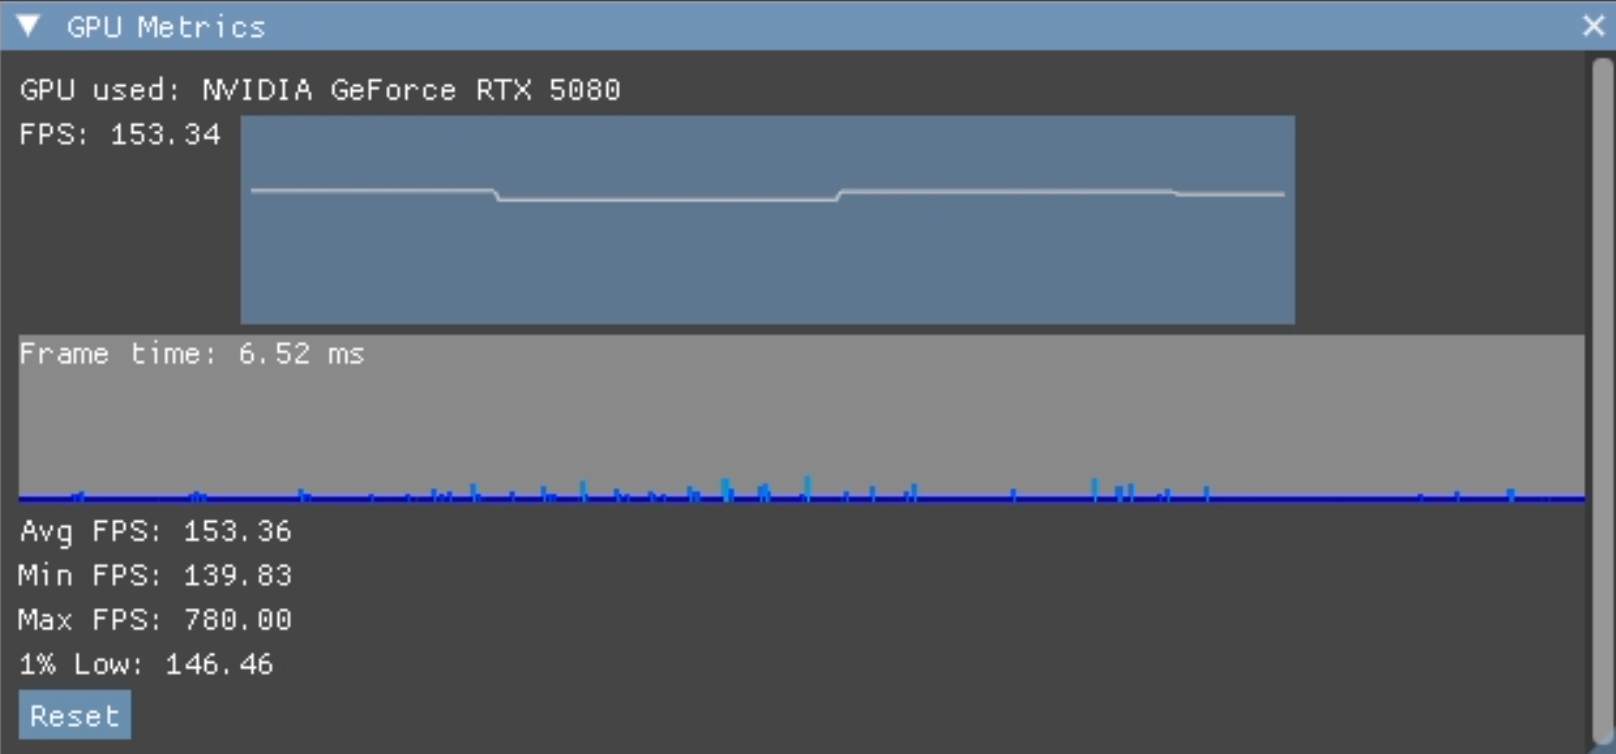
\includegraphics[width=\textwidth]{images/5080-linux-1.png}
        \caption{Ubuntu Benchmark 2 \\ \hspace*{6em} RTX 5080 16 GB}
        \label{fig:5080-linux-test-1}
    \end{minipage}
\end{figure}

\begin{figure}[ht]
    \centering
    \begin{minipage}[b]{0.48\textwidth}
        \centering
        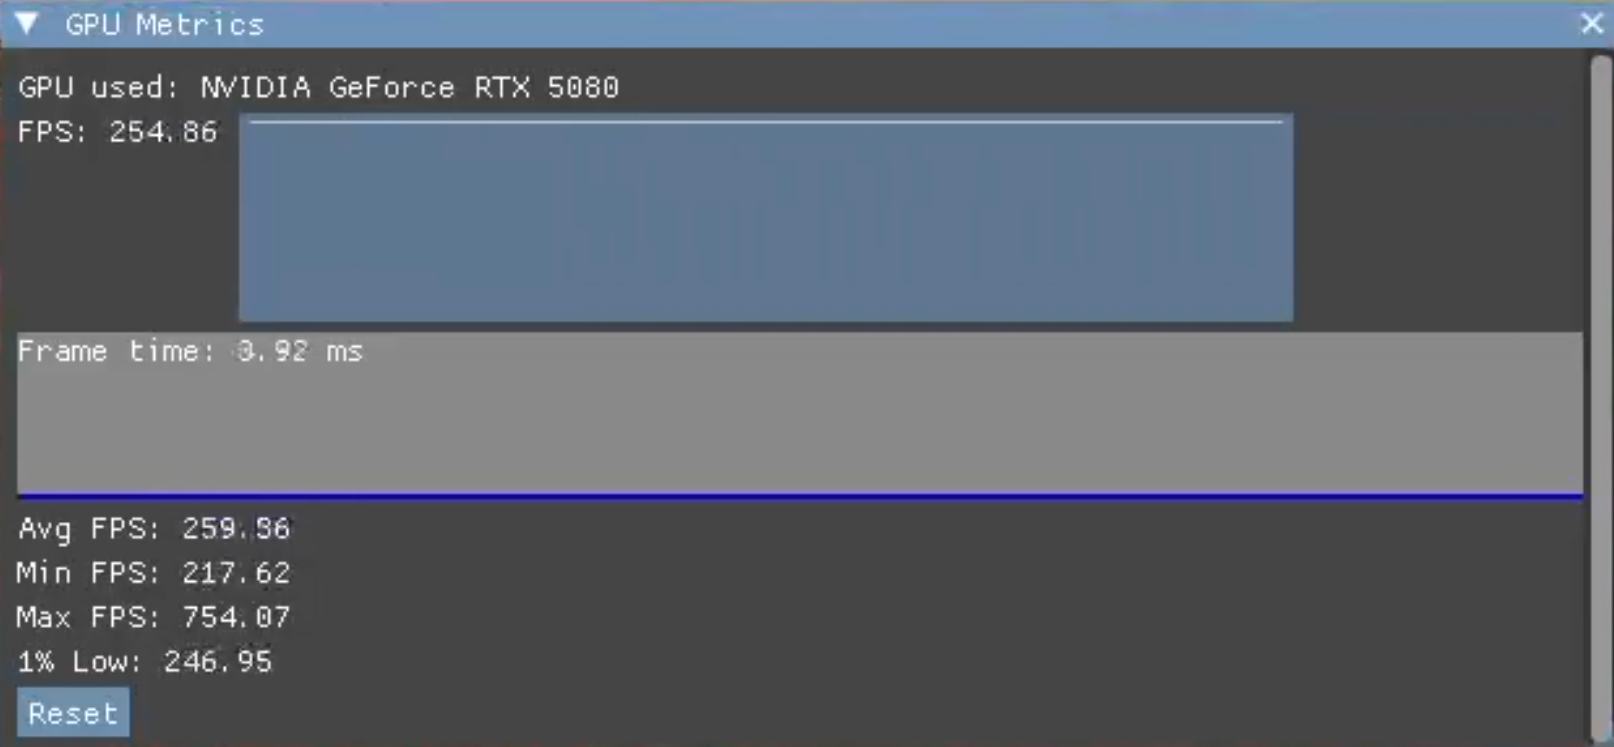
\includegraphics[width=\textwidth]{images/5080-windows-2.png}
        \caption{Windows Benchmark 2 \\ \hspace*{6em} RTX 5080 16 GB}
        \label{fig:5080-windows-test-2}
    \end{minipage}
    \hfill
    \begin{minipage}[b]{0.48\textwidth}
        \centering
        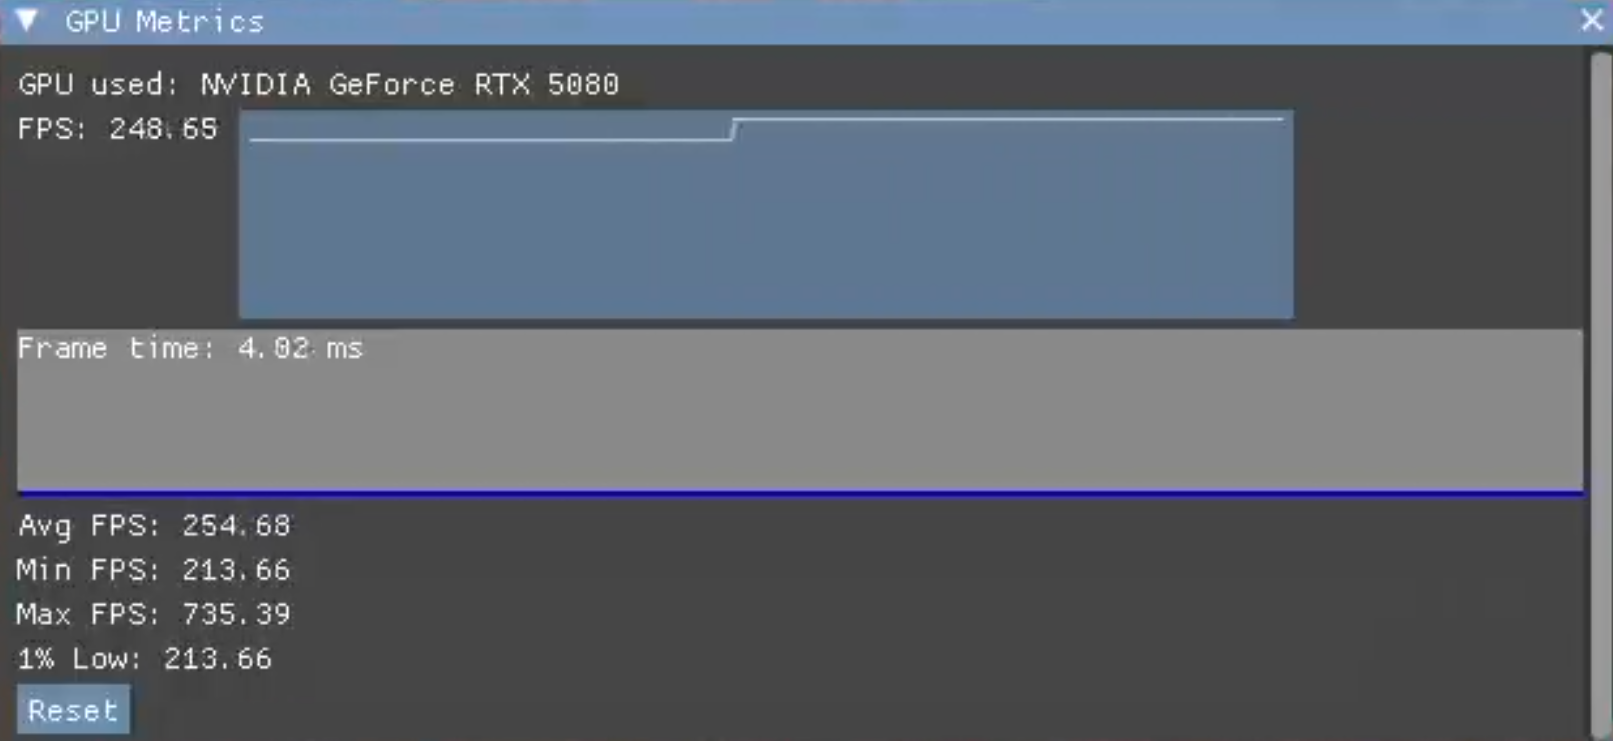
\includegraphics[width=\textwidth]{images/5080-linux-2.png}
        \caption{Ubuntu Benchmark 2 \\ \hspace*{6em} RTX 5080 16 GB}
        \label{fig:5080-linux-test-2}
    \end{minipage}
\end{figure}

Ultima comparație constă în prezentarea rezultatelor unui singur benchmark cu un număr variat de particule, rulate pe Windows 10 (\autoref{fig:laptop-non-test-2}, \autoref{fig:laptop-opt-test-2}), dar cu o configurație hardware modestă: procesor AMD Ryzen 5 3500U 3.7 GHz, 8GB RAM DDR4 2400 MHz, AMD Radeon Vega 8. Aceste teste folosesc o placă video integrată, iar asta scade drastic performanța întregului sistem de particule. În Benchmark 2, cu 8.388.608 de particule, aplicația este aproape imposibil de utilizat, având un FPS mult sub pragul necesar pentru \textit{Real-Time Rendering}. Împărțind numărul inițial de particule la 32, cu un total de 262.144, putem ajunge din nou la un FPS acceptabil, puțin sub obiectivul actual de 60 FPS, standardul minim pentru a obține o experiență fluidă în grafica pe calculator. O placă video integrată nu poate face față unui flux atât de mare de lucru și informații. Prin urmare, folosirea unei plăci video dedicate aduce într-adevăr îmbunătățiri semnificative de performanță față de una integrată. 

\begin{figure}[ht]
    \centering
    \begin{minipage}[b]{0.48\textwidth}
        \centering
        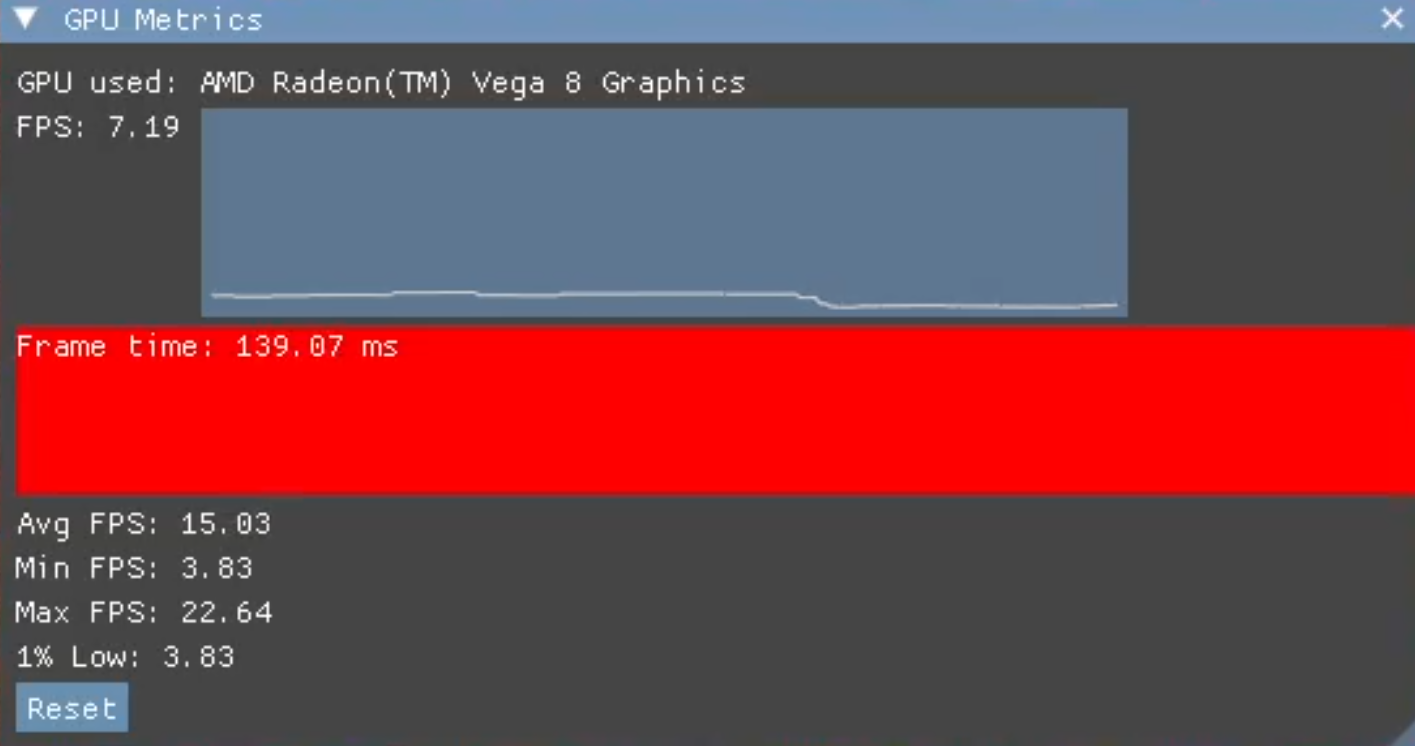
\includegraphics[width=\textwidth]{images/laptop-non-2.png}
        \caption{Windows - 8.388.608 particule \\ \hspace*{6em} AMD Radeon Vega 8}
        \label{fig:laptop-non-test-2}
    \end{minipage}
    \hfill
    \begin{minipage}[b]{0.48\textwidth}
        \centering
        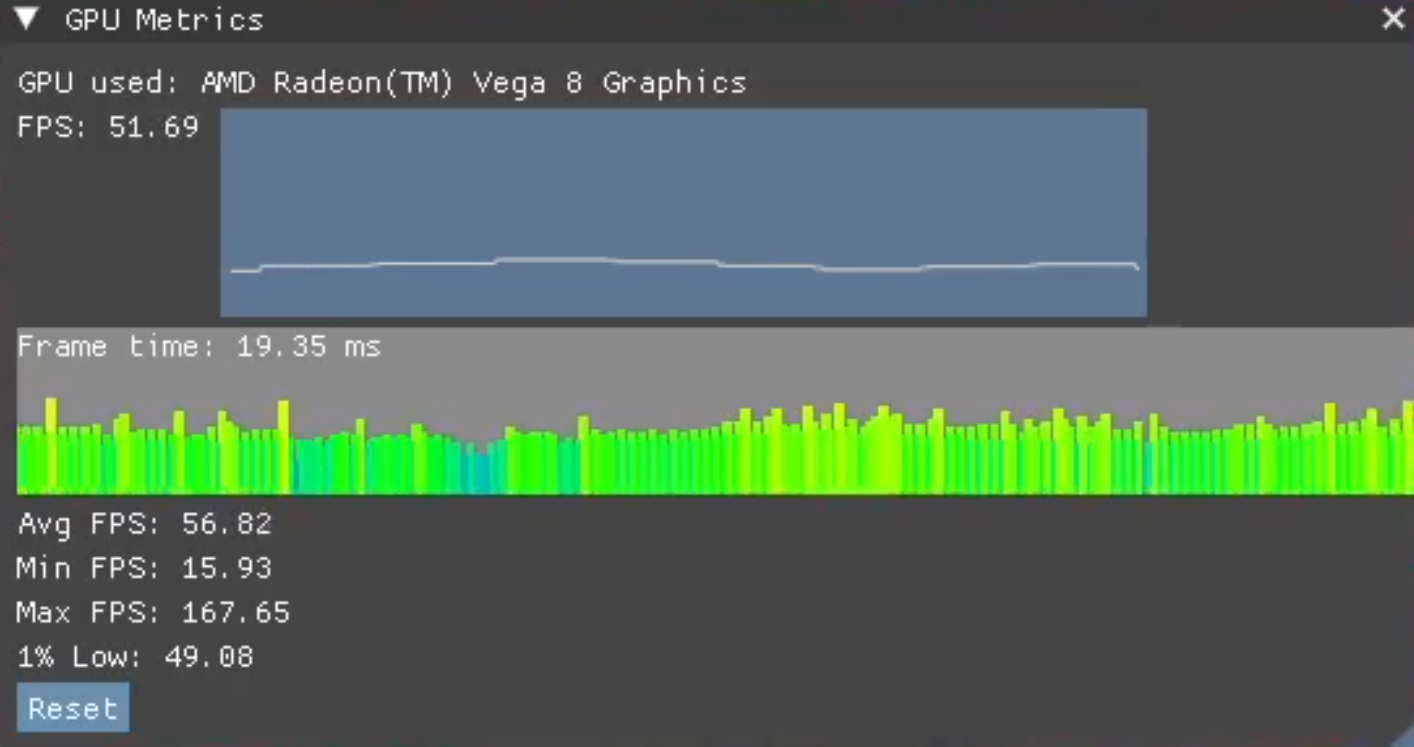
\includegraphics[width=\textwidth]{images/laptop-opt-2.png}
        \caption{Windows - 262.144 particule \\ \hspace*{6em} AMD Radeon Vega 8}
        \label{fig:laptop-opt-test-2}
    \end{minipage}
\end{figure}

\autoref{tab:benchmark1+2-table} și \autoref{tab:benchmark-particle-table} centralizează toate rezultatele testelor prezentate anterior. 

% ============================================================================================================
\section{Limitări}
% ============================================================================================================
Una dintre principalele limitări ale sistemului de particule este nevoia unei plăci video dedicate sau integrate, suficient de nouă și actualizată pentru a oferi suport complet pentru API-ul Vulkan. În urma testelor efectuate, o altă limitare semnificativă este legată direct de capacitatea hardware-ului folosit. Cu cât acesta este mai capabil, cu atât sistemul poate fi scalat și extins, fără să compromită performanța sau calitatea vizuală. Această constrângere este comună în cazul aplicațiilor cu un nivel ridicat de procesare computațională, unde creșterea complexității calculelor necesită resurse hardware proporțional mai puternice. 

% ============================================================================================================
\section{Direcții posibile pentru evoluția temei abordate}
% ============================================================================================================
Proiectul de față este un punct de plecare foarte bun pentru a crea un sistem de particule mult mai complex și mai spectaculos din punct de vedere grafic, capabil să simuleze cu un grad ridicat de realism diferite fenomene fizice și efecte vizuale. Se poate face tranziția la un sistem de particule în 3D și la simularea unor fenomene fizice complexe precum simularea materialelor textile, focului, fumului, lichidelor. Un alt obiectiv important ar fi integrarea unui sistem care să permită utilizatorilor să definească comportamentul particulelor prin shaders personalizabile. Acest lucru ar putea fi realizat prin intermediul unui editor integrat în aplicație, care să includă funcționalități de hot-reload pentru shaders, permițând compilarea acestora on-the-fly, fără a mai fi necesar recompilarea întregii aplicații pentru a reflecta noile modificări aduse fișierelor care definesc comportamentul pentru diferite shaders: compute, vertex, fragment. Un alt aspect interesant, care trebuie luat în calcul, este suportul pentru mai multe platforme. API-ul Vulkan permite integrarea aplicației și pe macOS sau iOS prin utilizarea MoltenVK \cite{MoltenVK_citation}, un subset al API-ului Vulkan peste framework-ul grafic Metal dezvoltat de Apple exclusiv doar pentru produsele sale. O altă platformă care include suport pentru Vulkan și pentru care ar putea fi extinsă aplicația curentă, este Android. Nu în ultimul rând, un aspect crucial al aplicației este dat de alegerea API-ului grafic folosit în implementare. Orice API are puncte forte și arii în care excelează, în funcție de arhitectura hardware-ului și cerințele aplicației. Un alt API poate oferi avantaje în anumite contexte, cum ar fi optimizari specifice pentru un sistem de operare și componentele hardware din spate. De aceea, introducerea și implementarea altor API-uri grafice moderne, în special DirectX 12 Ultimate \cite{DireX12Ultimate_citation} și Metal \cite{Metal_citation}, ar putea aduce noi perspective asupra tehnicilor de optimizare și arhitecturii folosite. 

% ============================================================================================================
% TABELE
% ============================================================================================================
\newpage
\vspace*{\fill}

\begin{table}[!ht]
\makebox[\textwidth][c]{
    \begin{NiceTabular}{|l|l|l|l|l|l|} 
    \hline
    \Block[c]{2-1}{Configurație Hardware} & \Block[c]{2-1}{Indicator}     &           \Block[c]{1-2}{Benchmark 1} &         &         \Block[c]{1-2}{Benchmark 2} &           \\ 
    \cline{3-6}
                                          &                               & Windows 11             & Ubuntu 24              & Windows 11             & Ubuntu 24              \\ 
    \hline
    \Block[c]{4-1}{GTX 1060 6GB}          & \rowcolor{blue!10} AVG FPS    & \Block[c]{1-1}{\textbf{92.03}}  & \Block[c]{1-1}{90.74}  & \Block[c]{1-1}{82.92}  & \Block[c]{1-1}{82.30}  \\ 
                                          & \rowcolor{green!10} MIN FPS   & \Block[c]{1-1}{80.15}  & \Block[c]{1-1}{88.72}  & \Block[c]{1-1}{\textbf{74.63}}  & \Block[c]{1-1}{80.36}  \\ 
                                          & \rowcolor{yellow!15} MAX FPS  & \Block[c]{1-1}{124.42} & \Block[c]{1-1}{124.11} & \Block[c]{1-1}{\textbf{199.54}} & \Block[c]{1-1}{145.07} \\ 
                                          & \rowcolor{red!10} 1\% Low FPS & \Block[c]{1-1}{80.15}  & \Block[c]{1-1}{\textbf{88.72}}  & \Block[c]{1-1}{74.63}  & \Block[c]{1-1}{80.36}  \\ 
    \hline
    \Block[c]{4-1}{RTX 5080 16GB}         & \rowcolor{blue!10} AVG FPS    & \Block[c]{1-1}{154.96} & \Block[c]{1-1}{153.36} & \Block[c]{1-1}{\textbf{259.36}} & \Block[c]{1-1}{254.68} \\ 
                                          & \rowcolor{green!10} MIN FPS   & \Block[c]{1-1}{139.89} & \Block[c]{1-1}{139.83} & \Block[c]{1-1}{\textbf{217.62}} & \Block[c]{1-1}{213.66} \\ 
                                          & \rowcolor{yellow!15} MAX FPS  & \Block[c]{1-1}{\textbf{784.77}} & \Block[c]{1-1}{780.00} & \Block[c]{1-1}{754.07} & \Block[c]{1-1}{735.39} \\ 
                                          & \rowcolor{red!10} 1\% Low FPS & \Block[c]{1-1}{147.57} & \Block[c]{1-1}{146.46} & \Block[c]{1-1}{\textbf{246.95}} & \Block[c]{1-1}{213.66} \\
    \hline
    \end{NiceTabular}
}
\caption{Comparație performanță Benchmark 1 și 2}
\label{tab:benchmark1+2-table}
\end{table}

\begin{table}[!ht]
\centering
\begin{NiceTabular}{|l|l|l|l|} 
\hline
\Block[c]{2-1}{Configurație Hardware}   & \Block[c]{2-1}{Indicator}     &           \Block[c]{1-2}{Particule} &           \\ 
\cline{3-4}
                                        &                               & 8.388.608              & 262.144              \\ 
\hline
\Block[c]{4-1}{AMD Radeon Vega 8}       & \rowcolor{blue!10} AVG FPS    & \Block[c]{1-1}{15.03}  & \Block[c]{1-1}{56.82}  \\ 
                                        & \rowcolor{green!10} MIN FPS   & \Block[c]{1-1}{3.83}  & \Block[c]{1-1}{15.93}  \\ 
                                        & \rowcolor{yellow!15} MAX FPS  & \Block[c]{1-1}{22.64} & \Block[c]{1-1}{167.65} \\ 
                                        & \rowcolor{red!10} 1\% Low FPS & \Block[c]{1-1}{3.83}  & \Block[c]{1-1}{49.08}  \\ 
\hline
\end{NiceTabular}
\caption{Comparație cu un număr diferit de particule}
\label{tab:benchmark-particle-table}
\end{table}

\vspace*{\fill}

% ============================================================================================================
% TODO
% ============================================================================================================
